\documentclass[12pt,a4paper]{article}

%\pdfoutput=1

\usepackage[utf8]{inputenc}
\usepackage[T1]{fontenc}
\usepackage[english]{babel}
\usepackage{amsmath}
\usepackage{mathabx}
\usepackage{lmodern}
\usepackage{dcolumn}
\usepackage{units}
\usepackage{siunitx}
\usepackage{icomma}
\usepackage{graphicx}
\usepackage{caption}
\usepackage{subcaption}
\usepackage{color}
\usepackage{pgf}
\DeclareMathOperator{\acosh}{arccosh}
\newcommand{\N}{\ensuremath{\mathbbm{N}}}
\newcommand{\Z}{\ensuremath{\mathbbm{Z}}}
\newcommand{\Q}{\ensuremath{\mathbbm{Q}}}
\newcommand{\R}{\ensuremath{\mathbbm{R}}}
\newcommand{\C}{\ensuremath{\mathbbm{C}}}
\newcommand{\rd}{\ensuremath{\mathrm{d}}}
\newcommand{\id}{\ensuremath{\,\rd}}
\usepackage{hyperref}
%\usepackage{a4wide} % puts the page numbering further down the page.
\usepackage{pdfpages}
\usepackage{epstopdf}
\DeclareGraphicsExtensions{.eps}

\title{Low Noise Amplifier Design}
\author{Marcus Malmquist, marmalm}
\date{\today}

\begin{document}
\maketitle

\section{Workflow}\label{sec:wf}
I wrote a Python-script to numerically solve this task. The workflow of the program can be seen in Figure~\ref{fig:workflow}. It is probably easier to understand the code after looking at the workflow graph.
\begin{figure}[h]
  \centering
  \noindent\makebox[\textwidth]{\scalebox{0.7}{\input{figures/flow_chart.pdf_t}}}
  \caption{The workflow of the program that wss used to design the LNA. It starts from the top and works its way down, following the appropriate arrows, until it reaches the end.}
  \label{fig:workflow}
\end{figure}

\section{LNA Design}
The starting values for $\Gamma_S$ and $\Gamma_L$ was chosen to be $\Gamma_\text{opt}$ and $\Gamma^*_\text{out}$ respectively. The reason I choose these starting values is because according to (12.53) in Pozar the noise figure of the amplifier is minimized when $Y_S=Y_\text{opt}$ which in turn means that $\Gamma_S=\Gamma_\text{opt}$ and because the gain is maximized when $\Gamma_L=\Gamma^*_\text{out}$.

The output and the final values can be seen in Figure~\ref{fig:result}. These values assumes that the system impedance is $\SI{50}{\ohm}$.
\begin{figure}[h]
  \centering
  \noindent\makebox[\textwidth]{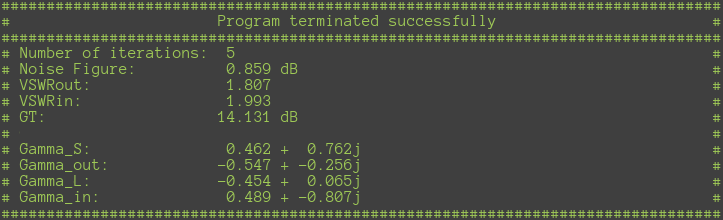
\includegraphics[width=\textwidth]{figures/result.png}}
  \caption{Output from the program after successful termination.}
  \label{fig:result}
\end{figure}

The matching networks can be seen in Figure~\ref{fig:mnt}.
\begin{figure}[h]
  \centering
  \noindent\makebox[\textwidth]{\scalebox{0.7}{\input{figures/mnt.pdf_t}}}
  \caption{Output and input matching network.}
  \label{fig:mnt}
\end{figure}
\end{document}